\documentclass[11pt]{article}
\usepackage[utf8]{inputenc} % Para caracteres en espa�ol
\usepackage{amsmath,amsthm,amsfonts,amssymb,amscd}
\usepackage{multirow,booktabs}
\usepackage[table]{xcolor}
\usepackage{fullpage}
\usepackage{lastpage}
\usepackage{enumitem}
\usepackage{floatrow}
\usepackage{multicol}
\usepackage{fancyhdr}
\usepackage{mathrsfs}
\usepackage{wrapfig}
\usepackage[final]{pdfpages}
\usepackage{setspace}
\usepackage{esvect}
\usepackage{calc}
\usepackage{multicol}
\usepackage{cancel}
\usepackage{graphicx}
\graphicspath{ {picturesB/} }
\usepackage[retainorgcmds]{IEEEtrantools}
\usepackage[margin=3cm]{geometry}
\usepackage{amsmath}
\newlength{\tabcont}
\setlength{\parindent}{0.0in}
\setlength{\parskip}{0.05in}
\usepackage{empheq}
\usepackage{framed}
%\usepackage{newtxmath}
\usepackage{euscript}
\DeclareMathAlphabet{\mathpzc}{T1}{pzc}{m}{it}
\usepackage[most]{tcolorbox}
\usepackage{xcolor}
\colorlet{shadecolor}{orange!15}
\parindent 0in
\parskip 12pt
\geometry{margin=1in, headsep=0.25in}
\theoremstyle{definition}
\newtheorem{defn}{Definition}
\newtheorem{reg}{Rule}
\newtheorem{exer}{Exercise}
\newtheorem{note}{Note}
\newcommand{\volume}{{\ooalign{\hfil$V$\hfil\cr\kern0.08em--\hfil\cr}}}
\newcommand{\parr}{\mathbin{\|}} % Parralel Symbol
\begin{document}
\setcounter{section}{2}%Section we want -1
\setcounter{page}{51} %Page we want
\setcounter{equation}{78}%Equation we want -1
\def\thepart{\arabic{part}}
\setcounter{part}{9}
\numberwithin{equation}{part}

 \pagestyle{fancy}
\fancyhf{}
\rhead{Section 9:  Electrostatic Propulsion - Electrospray/Colloid Thrusters}
\rfoot{Page \thepage}
\thispagestyle{empty}

\begin{center}
{\LARGE \bf Section 9:  Electrostatic Propulsion}\\
{\large AE435}\\
Spring 2018
\end{center}
\vspace{5mm}
\section{Electrospray/Colloid Thrusters}
\vspace{25mm}
\tableofcontents
\newpage
Electrospray/colloid propulsion different from ion thruster and HET, but still electrostatic propulsion.  Main difference = liquid propellant, not noble gas (xenon).
 
In electrospray/colloid propulsion charged particles are extracted from a liquid and accelerated to high speed.  These particles are generally not individual atoms (not Xe+ or Li+), but are typically molecular species (e.g., 1-Ethyl-3-methylimidazolium a.k.a. Emim+ or BF4-  tetrafluoroborate) and cluster/droplets of those species (e.g., many hundreds of molecules bonded together within a droplet, which likely has charge-state >1)
 
Three main types of technologies, based on the type of liquids and type of emission:
\begin{enumerate}
\item Colloid thruster - accelerates and expels charged droplets, and uses solvents such as glycerol and formamide as propellant
\item Field emission electric propulsion (FEEP) - uses liquid metals (Cs and In) to emit positively charged metal ions
\item Ionic liquid ion sources (ILIS) - room-temperature molten salts (i.e., "ionic liquids") used to create ion beams (individual molecular ion emission) or mixtures of ions with droplets.  No need to ionize, free charges already present in the liquid.
 \end{enumerate}
Electrospray well-known in chemistry and materials analysis community.  Electrospray ionization used in mass spectrum analysis to study liquids.  Ions/droplets extracted from liquid and mass spectrum analyzed, usually for bio-related materials, e.g., proteins, prescription drugs.
 
  \begin{center}
{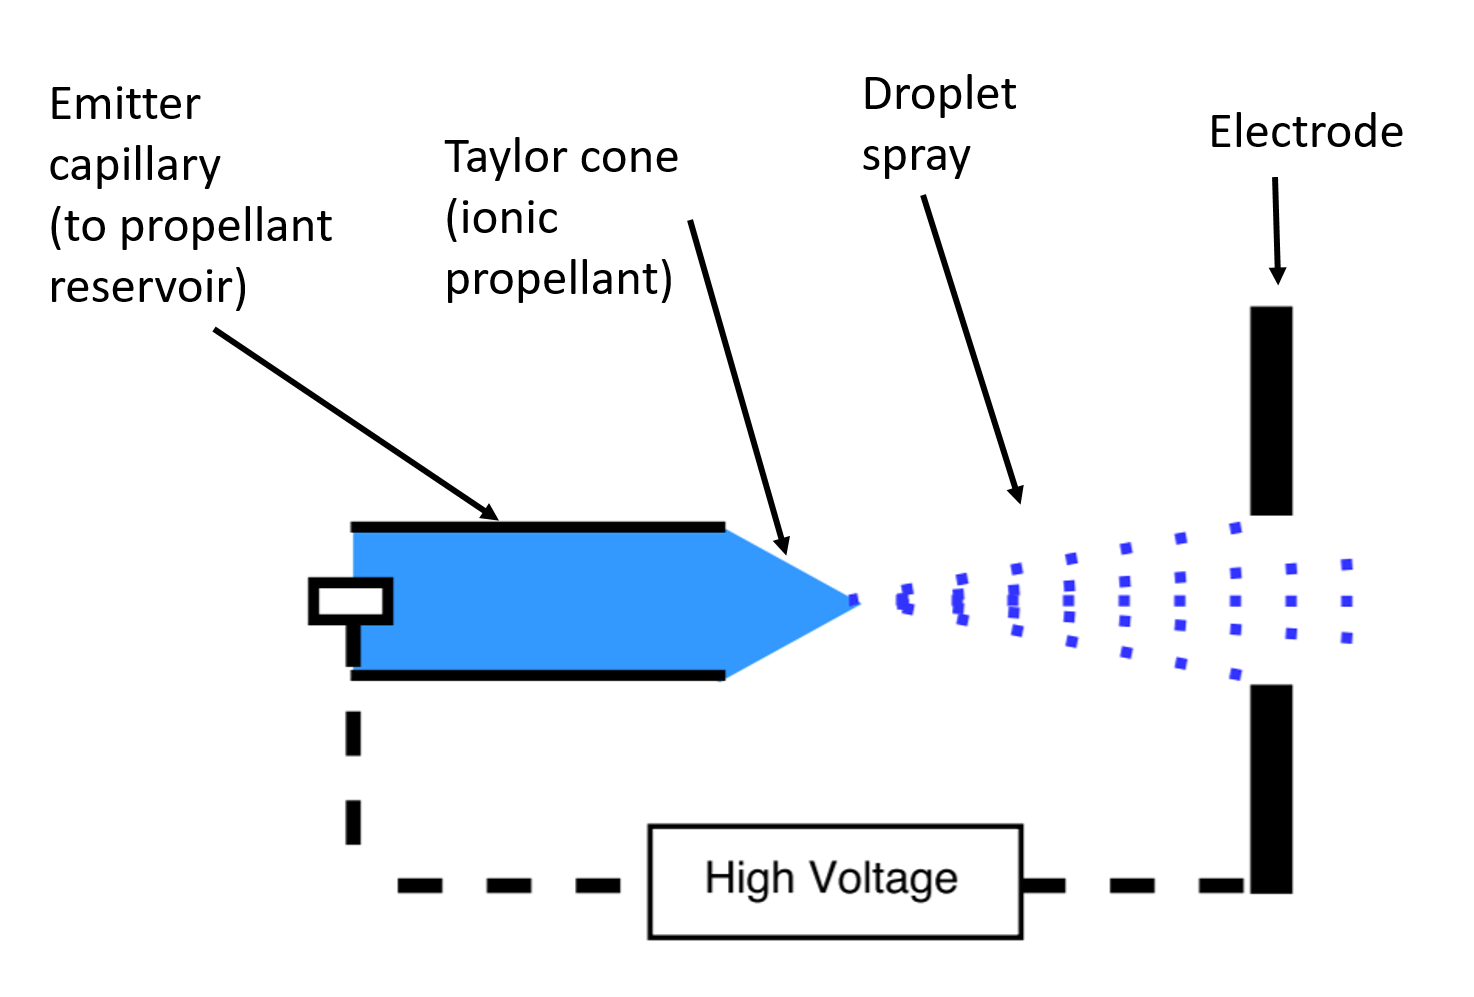
\includegraphics[scale=0.9]{31.png}}
\end{center}
%These propellants can conduct adnw e are extrating out the ions at the tip. , being accelerated by the electric field. The m
 \begin{center}
{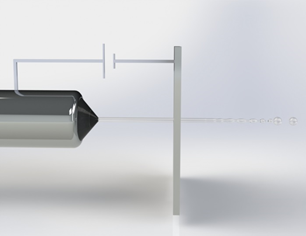
\includegraphics[scale=1]{32.png}}
\end{center}

\subsubsection{Motivation for Electrospray Propulsion}
%Samll packaging, possibly better efficiency becasue you dont have to pay any ionization cost. 
High thrust-density.

Remember we are converting electric potential energy to kinetic energy. 
   \begin{equation}
 \begin{aligned}
 q \, V_{acc} = \frac{1}{2} Mv^2 \quad \rightarrow \quad V_{accel} = \frac{Mv^2}{2q}
 \end{aligned}
 \end{equation}
 
Thrust can be written as ...
   \begin{equation*}
 \begin{aligned}
 T = \dot{m}_i \, v_i = \frac{I_bM}{e} \, \sqrt{\frac{2eV}{M}} 
 \end{aligned}
 \end{equation*}
 
And with the beam current that is space charge limited, running the electrospray at it maximum possible current...
  \begin{equation*}
 \begin{aligned}
 I_{b,scl} = \frac{4}{9} \, \varepsilon_o \, \sqrt{\frac{2e}{M}} \, \frac{V^{\frac{3}{2}}}{d^2} A
 \end{aligned}
 \end{equation*}
 
 Then we can write thrust per unit area as...
   \begin{equation}
 \begin{aligned}
 \frac{T}{A} = \frac{8}{9} \, \varepsilon_o \, \bigg(\frac{V}{d}\bigg)^2
 \end{aligned}
 \end{equation}
 
If we want higher thrust density, we have to have a higher voltage soooo we look at 9.79. If we want higher voltage we can have higher M or higher v, exit velocity which is related to ISP which is related to the delta V. So we can think in equation 9.79, v is set by whatever mission we want to do. We must increase M/q then, this is all we can change. In other words....
 
Also remember the mission delta-v will dictate the optimum particle velocity, v, so v = constant for given mission.  To get higher thrust-density (more thrust in smaller package) want higher voltage per (9.80).   Then per (9.79) higher voltage requires higher mass-to-charge (m/q) ratio.  Hence why we want singly-charged xenon in ion thruster (131.1 amu, or why early ion thrusters used mercury 201 amu, and why Hall thrusters have experimented with Bismuth 209 amu, higher thrust density).  So instead of emitting atomic ion, emit polyatomic ion (e.g., Emim+  146 amu/q for single ion, or droplet with thousands of polyatomic molecules, m/q huge!, for example droplet m/q values of 1024 amu/q)
 
Also, higher accelerating voltage reduces cost-of-ion voltage losses, as we saw in (9.35):
 
   \begin{equation}
 \begin{aligned}
 \eta = R = \frac{V_b}{V_s + |V_a|} = \frac{V}{V + V_{loss}}
 \end{aligned}
 \end{equation} %The accelerator grid is a los, its a negative, if V is reallt large this goes to 1. As V increases, efficicneyt increse. We would like to not have the acceleration loss but thats not possible for ION thrusters.
 
Would like $V_a$ equal zero.  (remember, accelerator grid voltage is below space potential, doesn't help accelerate the ions, below space potential to keep electrons from backstreaming).
 
So, higher m/q means higher voltage, less voltage loss (better efficiency), and higher thrust density.  BUT, don't want the voltage too high (No M/q to large)!  For example, for mission requiring 1000 sec Isp, an m/q of 1024 amu/q means 100kV accelerating voltage!  Yikes!
 
So the potential benefits are high-thrust density, low thrust, small packaging/volume, and these types of propulsion have been explored mainly most recently for small/CubeSats.


  \begin{center}
{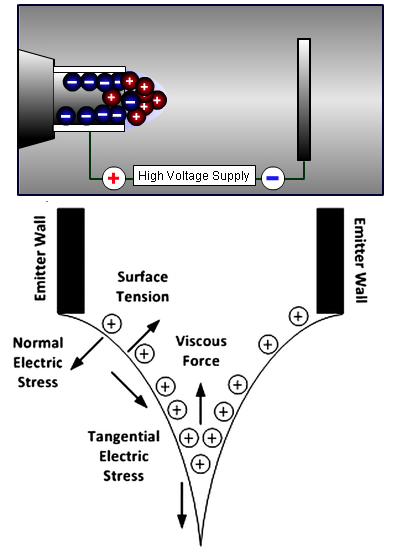
\includegraphics[scale=.65]{37.png}}
\end{center}

\subsection{Liquid Surface Physics}
We are interested in how a liquid surface responds to an applied strong normal electric field, $E_o$.
 

First consider the interface between vacuum and a conductive liquid (liquid with free charges, ions in it).
 \begin{center}
 \vspace{30mm}
 \textbf{Figure:}
 \end{center}
 
 Gauss' Law $\rightarrow$
    \begin{equation}
 \begin{aligned}
\sigma = \varepsilon_o \, E_o
 \end{aligned}
 \end{equation}
    \begin{equation*}
 \begin{aligned}
\int \int_S \vv{E} \cdot \mathrm{d}\vv{A} = \frac{Q}{\varepsilon_o} = \frac{\sigma \, A}{\varepsilon_o}
 \end{aligned}
 \end{equation*}
 
But what if it's a dielectric liquid, with no free charges? Will get
polarization. The molecules of the liquid are now polarized (i.e.,
modeled as dipoles), and we need to account for the electric field
that will be due to these dipoles, the net Efield. That is, the
Displacement field? Eqn. (2.34). Now:
\begin{center}
 \vspace{30mm}
 \textbf{Figure:}
 \end{center}
    \begin{equation*}
 \begin{aligned}
\nabla \cdot \vv{D} = \rho_{free} = 0 \\ \\ 
\vv{D} = \varepsilon \, \vv{E} = \varepsilon_r \, \varepsilon_o \, \vv{E}
 \end{aligned}
 \end{equation*}
where
Relative permittivity (i.e., dielectric constant), we called it K in
(2.42), or $\varepsilon_r$. So...

    \begin{equation*}
 \begin{aligned}
\varepsilon \, \varepsilon_o \, E_o - \varepsilon \, \varepsilon_i \, E_i = \sigma_{free} = 0
 \end{aligned}
 \end{equation*}
    \begin{equation}
 \begin{aligned}
 \varepsilon_o \, E_o - \varepsilon \, \varepsilon_i \, E_i = \sigma_{free} = 0
 \end{aligned}
 \end{equation}
 
Also:
    \begin{equation*}
 \begin{aligned}
\nabla \cdot \vv{E} &= \frac{\rho_{free}}{\varepsilon_o} = \frac{1}{\varepsilon_o} \, \rho_{free} + \frac{1}{\varepsilon_o} \, \rho_{p} \\ \\
\rho_{free} &= 0 \rightarrow
 \end{aligned}
 \end{equation*}
 
     \begin{equation}
 \begin{aligned}
\int \int \vv{E} \cdot \mathrm{d}\vv{A} &= \frac{1}{\varepsilon_o} \, \rho_p = \frac{\sigma_p \, A}{\varepsilon_o} \\ \\
\quad &\rightarrow  \varepsilon_o \, E_o - \varepsilon \, \varepsilon_i \, E_i = \sigma_{p}
 \end{aligned}
 \end{equation}
where polarization (or dipole) charge density is $\sigma_p$

Combine (9.83) and (9.84) to show
    \begin{equation}
 \begin{aligned}
\sigma_p = (1 - \frac{1}{ \varepsilon}) \, \varepsilon_o \, E_o
 \end{aligned}
 \end{equation}
     \begin{equation}
 \begin{aligned}
E_i = \frac{1}{\varepsilon} \, E_o
 \end{aligned}
 \end{equation}
 
Note, if the dielectric constant (relative permitivitty) is high, then
(9.85) is the same as (9.82). The relationship between surface
charge density and electric field is same for dielectric liquid and
conductive liquid (if $\varepsilon \gg 1$). $\varepsilon \sim 80$ for typical electrospray liquids.

\subsubsection{Relaxation time}
The relaxation time is the characteristic time for charges or dipoles
within the liquid to respond/adjust to a change in the applied
electric field.

Conductive liquid with conductivity K, (Si/m). Efield is suddenly
applied, so charges within the liquid begin to move toward surface,
building up a surface charge density.

    \begin{equation}
 \begin{aligned}
\frac{\mathrm{d} \sigma}{\mathrm{d} t} = k \, E_i
 \end{aligned}
 \end{equation}

Relationship between applied field and the field in the liquid is
(9.83) with free charge density not = 0, so:

    \begin{equation*}
 \begin{aligned}
\frac{\mathrm{d} \sigma}{\mathrm{d} t} = k \, \bigg(\frac{\varepsilon_o \, E_o}{\varepsilon_o \, \varepsilon} - \frac{\sigma}{\varepsilon_o \, \varepsilon}\bigg)
 \end{aligned}
 \end{equation*}
 
     \begin{equation}
 \begin{aligned}
\frac{\mathrm{d} \sigma}{\mathrm{d} t} - \frac{k \sigma}{\varepsilon_o \varepsilon } = \frac{k \, E_o}{\varepsilon }
 \end{aligned}
 \end{equation}
 
 \newpage
Soln. of which for $\sigma(0) = 0$ is:

    \begin{equation}
 \begin{aligned}
\sigma(t) = \varepsilon_o \, E_o \, \bigg(1 - \exp\bigg(-\frac{t}{T}\bigg)\bigg)
 \end{aligned}
 \end{equation}
 
where relaxation time of charges in the liquid,
    \begin{equation}
 \begin{aligned}
T = \frac{\varepsilon \, \varepsilon_o}{k}
 \end{aligned}
 \end{equation}
 
 \begin{center}
 \vspace{50mm}
 \textbf{Figure: Relaxation Time of Charges in Propellant}
 \end{center}
 
\subsubsection{Stability of the Surface}
Consider a surface with a small perturbation (a small ripple) in
presence of applied field. The local Efield is concentrated at the
peaks of the ripple, intensifying the surface charge density and
corresponding Electric field at those peaks.
 \begin{center}
 \vspace{50mm}
 \textbf{Figure: Electric Field at Peaks}
 \end{center}
 
The electric field is pulling the fluid up with force per unit area
(pressure):

    \begin{equation}
 \begin{aligned}
P_{\text{Efield}} = \frac{F}{A} = \frac{1}{2} \sigma E = \frac{1}{2} \varepsilon_o \, E^2 
 \end{aligned}
 \end{equation}
 
The electric field pulling the fluid is counteracted by the surface
tension of the fluid. But as the Efield and force at the ripple
increases, the process can become unstable. So, we need to
determine the Efield at the surface (and corresponding force due to
the Efield from (9.91)), determine the surface tension restoring
force, and see when does Electric force overcome surface tension
and cause instability.

\subsubsection{Efield at Surface}

Assume sinusoidal surface ripple. Outside the fluid, the electric
potential obeys Laplace eqn., with the potential going to zero at the
surface. This potential near the vicinity of the surface can be
written as superposition of applied field and a small perturbation.
    \begin{equation}
 \begin{aligned}
a
 \end{aligned}
 \end{equation}
The small perturbation varies sinusoidal in x-direction, and decays
exponentially in y-direction. Then Electric field at surface is:
    \begin{equation}
 \begin{aligned}
a
 \end{aligned}
 \end{equation}
for and on the crests of the ripple, where the Efield is
strongest
Finally, recognize we are interested in the change in the Electric
force (pressure) on the charged liquid surface due to the small
ripple/perturbation. That is, with (9.91) and (9.93):
    \begin{equation}
 \begin{aligned}
a
 \end{aligned}
 \end{equation}

\subsubsection{Counteracting Surface Tension}

Force (or pressure) due to surface tension is:
\begin{shaded}
\textbf{Force Due to Surface Tension:}

    \begin{equation}
 \begin{aligned}
\frac{F}{A} = P_{\text{surface tension}} = \gamma \, \bigg(\frac{1}{R_x} + \frac{1}{R_y}\bigg)
 \end{aligned}
 \end{equation}
 
Where
\begin{itemize}
\vspace{-5mm}
\item $R_x$ and $R_y$ are the radii of curvature of the surface along the x and
y-directions for a two dimensional surface (would be x and
z-directions in the ripple figure above)
\item $\gamma$ Is the surface tension of the fluid (a fluid property)
\end{itemize}
\end{shaded}

For a cylindrically symmetric surface, this becomes:
    \begin{equation}
 \begin{aligned}
P_{\text{surface tension}} = \gamma \, \frac{2}{R_c}
 \end{aligned}
 \end{equation}
This surface curvature is related to the second derivative of the
surface of the fluid.
    \begin{equation*}
 \begin{aligned}
\frac{1}{R_c} \approx \bigg|\frac{\partial^2 y}{\partial x^2}\bigg|
 \end{aligned}
 \end{equation*}
We need a relationship between x and y at the surface. Recognize
that the surface is an equipotential line with zero potential at the
surface (9.92) $\rightarrow$
    \begin{equation}
 \begin{aligned}
a
 \end{aligned}
 \end{equation}
Then the surface tension storing force is:
\subsubsection{Instability}
Instability results if the force on the surface due to electric field
overcomes the restoring force of the surface tension. That is
(9.94) $>$ (9.97):
    \begin{equation}
 \begin{aligned}
a
 \end{aligned}
 \end{equation}
Wavelength of the ripple
where
So for long wavelength ripples, a weaker electric field can cause
instability. Similarly, liquids with lower surface tension require
weaker electric field to induce instability. In electrospray we are
generally working with capillary (small tubes with diameter D),
that have a corresponding longest wavelength of 2D, thus:
    \begin{equation}
 \begin{aligned}
a
 \end{aligned}
 \end{equation}
Consider a new multi-mode propellant consisting of HAN and
[Emim][EtSO4] with surface tension of 45 mN/m being
electrosprayed from a D = 100 micron capillary. The required
Efield is $1.26\times10^7$ V/m very high! (parallel plates separated by
5mm would require potential of 63kV!) But this analysis assumed
uniform applied E across large surface of liquid. In reality, the
Efield is applied between a downstream extractor plate, and the tip
of a needle/emitter. The Efield concentrates at the tip of the needle/emitter where the fluid surface is. So, in reality lower
voltages $\sim$1-3kV are possible to create these large Efields for
stability. A more detailed analysis of this extractor-needle/emitter
geometry follows.

 \newpage
\subsection{Taylor Cone}
\subsubsection{Electric Potential Profile/Structure}
Consider an emitter-extractor setup. What would we expect the
potential profile to look like?
\begin{center}
\vspace{70mm}
\textbf{Figure: Electric Potential Field Lines}
\end{center}
\subsubsection{Voltage to Cause Instability}
To better model the Efield/electric potential structure in a emitter-extractor
geometry, we use Prolate Spheroidal Coordinates.
 \begin{center}
{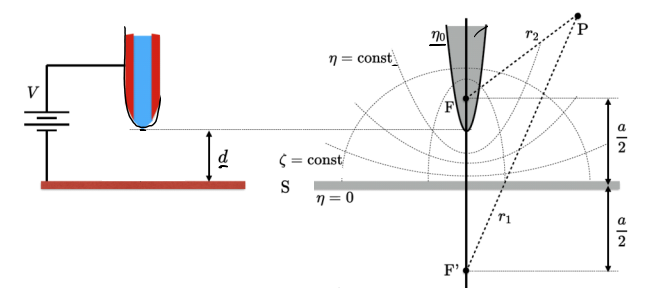
\includegraphics[scale=0.75]{33.png}}
\end{center}

\begin{framed}
Here
    \begin{equation}
 \begin{aligned}
\eta = \frac{r_1 - r_2}{a} \qquad \text{,} \qquad \xi = \frac{r_1 + r_2}{a}
 \end{aligned}
 \end{equation}
and conversion from cartesian-to-prolate coordinates is:
    \begin{equation}
 \begin{aligned}
r_1 &= \sqrt{x^2 + y^2 + \bigg(z^2 + \frac{a}{2}\bigg)^2} \\ \\
r_2 &= \sqrt{x^2 + y^2 + \bigg(z^2 - \frac{a}{2}\bigg)^2} \\ \\
 \end{aligned}
 \end{equation}
 
\begin{itemize}
\item Lines of constant $\eta$ confocal hyperboloids (with foci at F, F')
\item Lines of constant $\xi$ are confocal ellipsoids (with focis at F, F')
\item "confocal" means having the same foci.
\item S is plane of symmetry ($\eta$=0)
\item We choose a surface ($\eta$=$\eta_o$) to represent the surface of the
capillary with liquid tip.

    \begin{equation*}
 \begin{aligned}
\eta_o = \frac{2d}{a}
 \end{aligned}
 \end{equation*}

\end{itemize}
\end{framed}
Why use such a weird coordinate system?

Because the $\eta$ surfaces are approximately equipotential surfaces.
That is, each $\eta$ surface corresponds to a different electric potential,
so we can use this geometry to solve for the electric potential and
therefore electric field within this geometry.
\begin{subequations}

If the potential on the emitter/liquid ($\eta$=$\eta_o$) is assumed to be V
(volts), and the S plane ($\eta$=0) is ground (V=0).
Relation for $\eta_o$ in this coordinate system is:

    \begin{equation}
 \begin{aligned}
\eta_o = \frac{2d}{a} \qquad \text{or} \qquad \eta = \frac{2z}{a}
 \end{aligned}
 \end{equation}
 
where d and a are the dimensions in the figure above. Then the potential on lines of constant $\eta$ within the gap is:
 
     \begin{equation}
 \begin{aligned}
\phi (\eta) = V \, \frac{\tanh^{-1} \eta}{\tanh^{-1} \eta_o}
 \end{aligned}
 \end{equation}
\end{subequations}


The resulting Efield at the tip is:
\begin{shaded}
\textbf{Electric Field at the Tip}
    \begin{equation}
 \begin{aligned}
E_{\text{tip}} = \frac{-\frac{2V}{R_c}}{\ln\bigg(\frac{4d}{R_c}\bigg)}
 \end{aligned}
 \end{equation}
assuming d$\gg$Rc
Where
\begin{equation*}
\begin{aligned}
R_c &= \text{Radius of Curvature of the Tip, $\approx$ radius of needle} \\ 
V &= \text{Capillary/Emitter Voltage} \\ 
d &= \text{Gap Distance} \\ 
\end{aligned}
\end{equation*}
\end{shaded}

Finally, for the liquid-vacuum/gas interface to become unstable,
we require electric pressure (traction or force per unit area, that is,
pressure created by electric field force) on the surface to be greater
than surface tension (pressure of surface tension).

    \begin{equation*}
 \begin{aligned}
\frac{1}{2} \varepsilon_o \, E^2 > \gamma \frac{2}{R_c}
 \end{aligned}
 \end{equation*}
 
which with (9.103) we find that the voltage on the emitter/needle
(with grounded extractor plane S) is:
\begin{shaded}
    \begin{equation}
 \begin{aligned}
V > \sqrt{\frac{R_c \gamma}{\varepsilon_o}} \, \ln\bigg(\frac{4d}{R_c}\bigg)
 \end{aligned}
 \end{equation}
where

$R_c$ is radius of curvature of the surface, which is approximately
the radius of the capillary/hypodermic needle emitter.
\end{shaded}

Again considering a new multi-mode propellant consisting of HAN
and [Emim][EtSO4] with surface tension of 45 mN/m being $\gamma$
electro-sprayed from a 100 $\mu$m capillary with extractor located 5
mm downstream. Rc = 100/2=50 $\mu$m, d = 5 mm, we get starting
voltage must be greater than 3020 Volts. If extractor ground plane
is only 2.5mm downstream, this becomes 2209 V.

For a 50micron capillary with extractor 1mm downstream $\rightarrow$ 1800V. Our experiments with this exact geometry required 1800-2000V.
\newpage
\subsubsection{Resulting Conical Surface Structure - Taylor Cone}

Once the electric field and corresponding force overcomes the
surface tension, we expect the shape of the liquid-vacuum interface
to change from spherical to conical:

\begin{center}
\vspace{50mm}
\textbf{Figure: Conical Taylor Cone}
\end{center}

This new conical surface shape was investigated and explained
analytically by G.I. Taylor in 1965, hence it's typically referred to
as a "Taylor" cone or Taylor's cone.

In this new conical geometry, we still have the requirement that the
electric force on the surface (in normal direction!) must be
balanced by the surface tension.

So we need to explore the surface tension and electric field/force in
this new conical geometry.

Surface tension (9.95) requires we know the radius of curvature of
the surface. Along the generator of the cone (the line that forms its
surface), the curvature is zero. But perpendicular to the generator
it's non-zero. We can find this curvature perpendicular to the
generator using Meusnier's Theorem:
 \begin{center}
{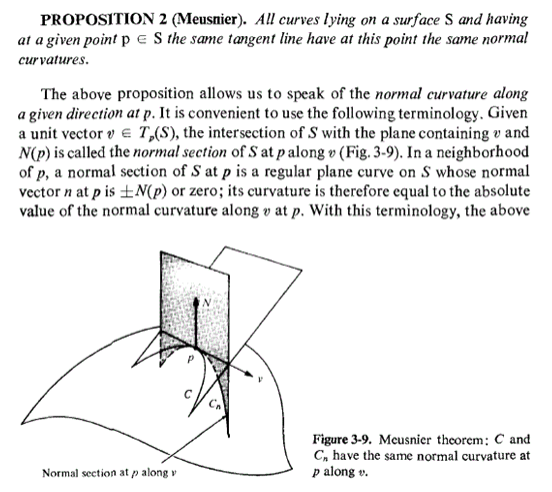
\includegraphics[scale=.7]{34.png}}
\end{center}
    \begin{equation*}
 \begin{aligned}
R &= R_c \cos \theta \\
R &= r \sin \theta \\
 \end{aligned}
 \end{equation*}
 so
     \begin{equation}
 \begin{aligned}
\frac{1}{R_c} = \frac{\cos \theta}{R} = \frac{\cos \theta}{r \sin \theta} = \frac{\cot \theta}{r}  \\
 \end{aligned}
 \end{equation}
 
     \begin{equation*}
 \begin{aligned}
\frac{1}{2} \varepsilon_o E_n^2 = \gamma \frac{1}{R_c} = \gamma \frac{\cot \theta}{r}
 \end{aligned}
 \end{equation*}
 
     \begin{equation}
 \begin{aligned}
E_n = \sqrt{\frac{2 \gamma \cot \theta}{\varepsilon_o r}}
 \end{aligned}
 \end{equation}

What type of electric potential profile will give us an Efield that
varies as (9.106), that is, falls off as $\sqrt{\frac{1}{r}}$?

Well, to calculate the potential outside the cone, we would use
Laplace Eqn. (2.22) because there is no charge outside the cone.
And the cone itself would be an equipotential surface. Further, we
may choose to work in spherical coordinates ($r$, $\theta$, $\phi$).

So we would solve Laplace Eqn. (2.22) in spherical coordinates.
This equation admits solutions that are Legendre functions of
either the first ($P_n$) or second ($Q_n$) kind. When n is a positive
integer these are referred to as "Legendre polynominals".
    \begin{equation*}
 \begin{aligned}
\phi \propto P_n (\cos \theta)r^n \qquad \text{and/or}\qquad \phi \propto Q_n (\cos \theta)r^n
 \end{aligned}
 \end{equation*}
Want electric field, so
    \begin{equation*}
 \begin{aligned}
E_n = E_{\theta} = -\frac{\partial \phi}{\partial \theta} \propto \frac{\partial }{\partial \theta} Q_n \sin \theta r^{n-1}
 \end{aligned}
 \end{equation*}
And we know Efield must have a $\frac{1}{\sqrt{r}}$ dependence, so $n = \frac{1}{2}$.

Unfortunately, these are Legendre functions of "fractional order".

    \begin{equation*}
 \begin{aligned}
\phi \propto P_{\frac{1}{2}} (\cos \theta)r^{\frac{1}{2}} \qquad \text{or}\qquad \phi \propto Q_{\frac{1}{2}} (\cos \theta)r^{\frac{1}{2}}
 \end{aligned}
 \end{equation*}

 \begin{center}
{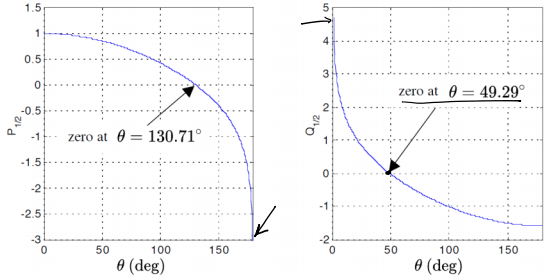
\includegraphics[scale=0.9]{35.png}}
\end{center}

The Legendre function of the 1st kind with fractional order 1/2  
($P_{\frac{1}{2}}$) has a singularity at pi (180$^{\circ}$). This is outside the cone in
free space where we are interested. The potential cannot go to
infinity there... not good, can't choose this one. But the Legendre
function of the 2nd kind with fractional order 1/2 ($Q_{\frac{1}{2}}$) has a
singularity at 0 (0$^{\circ}$). This is inside the cone, where our Laplace
solution would no longer be valid (of course, it's inside the liquid
where there are charges!)...so OK. Choose this one.

So we want     \begin{equation*}
 \begin{aligned}
Q_{\frac{1}{2}} \cos \theta
 \end{aligned}
 \end{equation*}

which has a zero (potential equals zero when $Q_{\frac{1}{2}} = 0$, this is the
liquid surface!) for an angle of 49.29$^{\circ}$. So the liquid
surface must have an angle of 49.29$^{\circ}$.

This is the angle of emission cone, or "Taylor" cone.

But what happens at the tip of the cone? 

As we move to the tip, $r \rightarrow 0$, what happens to the electric field (9.106)? Clearly
something must give? $E_n \rightarrow \infty$.

A jet will issue from the cone's tip, giving rise to a flow rate and,
since the surface being ejected is charged, a net current is also
emitted. "Cone-jet" mode.

 \begin{center}
{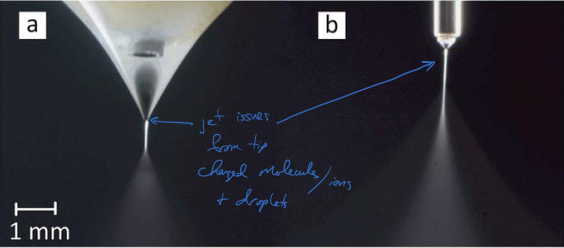
\includegraphics[scale=0.9]{36.png}}
\end{center}

\end{document}